\documentclass[10pt]{beamer}

%%%
% PREAMBLE FOR THIS DOC 
%%%
%https://tex.stackexchange.com/questions/68821/is-it-possible-to-create-a-latex-preamble-header
\usepackage{/Users/miw267/Repos/latex_preamble/beamer_preamble}

\usetikzlibrary{matrix}




%%%
% AGENDA TOPICS
%%%
\agendatopic[overview]{Overview: Three ways to prove implications}
\agendatopic[contrapositive]{Contrapositive: Details}
\agendatopic[contradiction]{Contradiction: Details}
\agendatopic[applications]{Applications}


%%%
% DOCUMENT
%%%

\begin{document}

%\maketitle

%% Title page frame
%\begin{frame}
%    \titlepage 
%\end{frame}





\title{10/9/2026: Contrapositive and contradiction}
\author{CSCI 246: Discrete Structures}
\date{Textbook reference: Sec 20, Scheinerman}

\begin{frame}
    \titlepage 
\end{frame}


\begin{frame}
\begin{myyellowbox}[title=Today's Agenda]
\begin{itemize}	
	\item Mini lecture ($\approx$  25 mins)
	\item Group exercises ($\approx$  25 mins)
\end{itemize}
\end{myyellowbox}
\vfill 
\end{frame}


%%%%%%%%%%%%%%%%%%%%
\agendaframe{overview}


\begin{frame}{There are three ways to prove $P \implies Q$.}

\colorbox{yellow!30}{\textbf{Poll.}} Suppose $P$ and $Q$ are propositions.  How can we prove $P \implies Q$?
\vfill
\pause 
\colorbox{red!30}{\textbf{Reminder.}} \qq{$P \implies Q$} is the same as \qq{If $P$, then $Q$.}
\vfill 
\pause 

\colorbox{green!30}{\textbf{Solution.}} There are three different strategies!
\begin{enumerate}
	\item \textbf{By direct proof.}   This is what we've been doing all along. See Proof Template 1, Scheinerman pp. 17. \pause 
	\item \textbf{By contraposition.}  We can prove $\lnot Q \implies \lnot P$.   \pause 
	\item \textbf{By contradiction.} We can assume  $\lnot (P \implies Q)$ and find a contradiction.  (Note: this is the same as assuming $P \land \lnot Q$ and finding a contradiction.)
\end{enumerate}	
\end{frame}


\begin{frame}{One claim, three proofs}


\colorbox{green!30}{\textbf{Claim.}}  Let $n$ be an integer. If $5n + 3$ is even, then $n$ is odd.

\vfill 
%\only<2->{\colorbox{red!30}{\textbf{Reference.}} \textbf{Direct proof}: Show $P \implies Q$.  \textbf{Contraposition}: Show $\lnot P \implies \lnot Q$.  \textbf{Contradiction}:  Show $P \land \lnot Q$ is impossible.}

\only<2->{
\begin{myredbox}[title=Reference] \textbf{Direct proof}: Show $P \implies Q$.  \textbf{Contraposition}: Show $\lnot P \implies \lnot Q$.  \textbf{Contradiction}:  Show $P \land \lnot Q$ is impossible.
\end{myredbox}
}
\vfill 
\only<3->{\colorbox{blue!30}{\textbf{Direct proof.}}}  \only<4->{Assume $5n+3$ is even, so $5n+3=2k$ for some integer $k$. Then $n = 2k - 4n - 3 = 2(k - 2n -2) + 1$, which is odd because $k - 2n - 2$ is an integer. $\blacksquare$} 

\vfill 
\only<5->{\colorbox{blue!30}{\textbf{By contraposition.}}}  \only<6->{The contrapositive is: if $n$ is even, then $5n+3$ is odd.  Let $n$ be even, so $n=2k$.  Then $5n+3=10k+3 = 2(5k+1)+1$, which is odd because $5k+1$ is an integer.$\blacksquare$} 

\vfill 
\only<7->{\colorbox{blue!30}{\textbf{By contradiction.}}}  \only<8->{Suppose, for contradiction, that $5n+3$ is even but $n$ is even.  Since $n$ is even, we write $n=2k$.  But then $5n+3=10k+3 =2(5k+1)+1$, which is odd.  So $5n+3$ is both even and odd, which is impossible. $\blacksquare$} 


\end{frame}

%%%%%%%%%%%%%%%%%%%%
\agendaframe{contrapositive}


\begin{frame}{Contraposition: Why does it work?}
\footnotesize 
\colorbox{yellow!30}{\textbf{Poll.}} How to show that the contrapositive technique works?
\vfill 

\only<2->{
\colorbox{yellow!30}{\textbf{Solution.}}
Recall that the truth table for the $\implies$ operator is given by  
\begin{center}
\begin{tabular}{cc|c}
P & Q & $\overbrace{P \implies Q}^{\text{If P, then Q}}$ \\
\hline 
\green{T} & \green{T} & \green{T} \\
\green{T} & \red{F} & \red{F} \\
\red{F} & \green{T} & \green{T}  \\
\red{F} & \red{F} & \green{T}  \\
\end{tabular}
\end{center}
}
\vfill 
\pause 
\only<3>{\alert{Now what}?}

\only<4->{Now we apply the $\implies$ operator to inputs transformed by the "\texttt{not}" operator (also written $\lnot$).
 \vspace{-.25cm}
\begin{table}
\centering
\begin{tabular}{cc|cc|c}
%\multicolumn{2}{c}{\textbf{Orig. props.}} & \multicolumn{3}{c}{\textbf{New props.}} \\
P & Q & $ \lnot Q$& $\lnot P$  & $\overbrace{\lnot Q \implies \lnot P}^{\text{If not Q, then not P}}$ \\
\hline 
T & T & \red{F}  & \red{F} & \green{T}\\
T & F & \green{T}  & \red{F} &  \red{F}  \\
F & T & \red{F}  &  \green{T}  &  \green{T}  \\
F & F & \green{T} & \green{T} & \green{T}
\end{tabular}
\end{table}
%
\vfill 
}

\vspace{-.25cm}
\only<5->{
\bluetextbox{The two tables have the same final column!}
}
\only<6->{
\bluetextbox{Hence $P \implies Q$ is equivalent to $\lnot Q \implies \lnot P$.}	
}
  

%\bluetextbox{Remark: We've shown that a proposition is logically equivalent to its contrapositive.  So what?  Sometimes it's easier to verify the contrapositive version.} 
\end{frame}





\begin{frame}{Contraposition: When should we use it?}
	
\only<1->{\colorbox{yellow!30}{\textbf{Poll.}} When should we use contraposition ($\lnot Q \implies \lnot P$)  instead of direct proof ($P \implies Q$)?}

\vfill 

\only<2->{\colorbox{green!30}{\textbf{Solution.}} Use contraposition when it's easier to work with the negation of the conclusion ($\lnot Q$) than with the assumption ($P$).}

\vfill 
 
 
\only<3->{\begin{mybluebox}[title=\text{Example: Prove the following claim.}]

\only<3->{\textbf{Claim}. Let $a,b$ be integers. If  $ab$ is even,  then $a$ is even or $b$ is even.}

\only<4->{\textbf{Contrapositive.} \pause If $a$ and $b$ are both odd, then $ab$ is odd.}

\vfill 


\only<5->{\textbf{Proof.} Write $a = 2k +1$ and $b=2 \ell + 1$. Then 
%
\begin{align*}
 ab &= (2k+1) (2 \ell+1) = 4k\ell+ 2k + 2 \ell + 1 \\
 &=2(2k\ell + k + \ell) + 1,
\end{align*}
which has the form 2m+1, i.e. odd. So the original claim holds.}	
\end{mybluebox}
}

\end{frame}


%%%%%%%%%%%%%%%%%%%%
\agendaframe{contradiction}



\begin{frame}{Contradiction: Why does it work?}

\begin{itemize}
\item \textbf{In general}: To prove proposition $R$, we can assume $\lnot R$ and find a contradiction. \pause 
\item \textbf{Specifically}: If we want to prove a proposition of the form $P \implies Q$, we can assume  $\lnot (P \implies Q)$ and find a contradiction. \pause 

	\vspace{.5cm}
	
	\colorbox{blue!30}{\textbf{Remark:}} Assuming  $\lnot (P \implies Q)$ is the same as assuming $P \land \lnot Q$.  \only<4>{\alert{Why?}}  \only<5->{To justify this, consider the truth table:
\begin{center}
\begin{tabular}{cc|c|c}
P & Q & $\overbrace{P \implies Q}^{\text{If P, then Q}}$ & $\lnot (P \implies Q)$\\
\hline 
\green{T} & \green{T} & \green{T} & \red{F} \\
\rowcolor{blue!20} % <--- shades this entire row
\green{T} & \red{F} & \red{F} & \green{T} \\
\red{F} & \green{T} & \green{T} & \red{F}  \\
\red{F} & \red{F} & \green{T} & \red{F} 
\end{tabular}
\end{center}
}
\end{itemize}

\only<6->{\colorbox{green!40}{\textbf{Conclusion.}} We can prove $P \implies Q$ by assuming $P \land \lnot Q$ and finding a contradiction.}
 	
\end{frame}



\begin{frame}{Contradiction: Another example}

\small 
\begin{mybluebox}[title=\text{Example: Prove the following claim.}]
\textbf{Claim.} If $n^2$ is even, then $n$ is even.
\pause
\vfill 
\textbf{Remark on logical structure.} We want to prove $P \implies Q$
where
\begin{itemize}
\item P: $n^2$ is even
\item Q: $n$ is even.	
\end{itemize}
\pause
\vfill 
\textbf{Proof by contradiction.} We assume $P \land \lnot Q$, where
\begin{itemize}
\item P: $n^2$ is even
\item $\lnot Q$: $n$ is odd.	
\end{itemize}
and derive a contradiction.
\pause
\vfill 
Now:
\begin{itemize}
	\item If $n$ is odd, write $n = 2k+1$. \pause 
	\item Then
	\[ n^2 = (2k+1)^2 = 4k^2 + 4k + 1 = 2(2k^2 + 2k) + 1, \]
	which is odd. \; $\Rightarrow\Leftarrow$
\end{itemize}


%This contradicts $P$, which assumed $n^2$ is even.
%Therefore

\end{mybluebox}


\end{frame}


\agendaframe{applications}


\begin{frame}{Machine learning: Why gradient descent stops}
\footnotesize
\begin{columns}[T]
\begin{column}{0.38\textwidth}
\centering
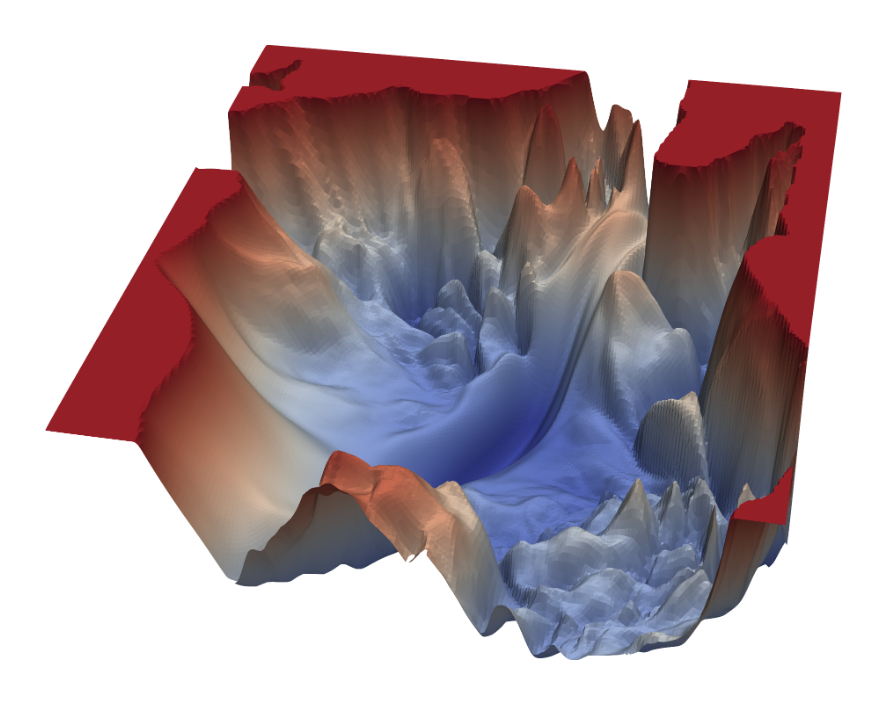
\includegraphics[width=\linewidth]{images/nonconvex_loss.png}

\scriptsize A nonconvex loss surface for a neural network: many local minima and saddle points where gradient descent can stop.  \\
\vspace{0.5cm}
\textit{Source:} H.~Li, Z.~Xu, G.~Taylor, C.~Studer, \& T.~Goldstein, ``Visualizing the Loss Landscape of Neural Nets,'' \textit{NeurIPS} 2018.
\end{column}


\begin{column}{0.6\textwidth}


\colorbox{yellow!30}{\textbf{Fact.}}   If $x$ is a local minimum of a differentiable function $f$, then $\nabla f(x) = 0.$ \\

\vspace{0.5cm} 
\pause 

\colorbox{yellow!30}{\textbf{Contrapositive.}} If $\nabla f(x) \neq 0$, then $x$ is not a local minimum, so you can still improve by stepping downhill. \\


\vspace{0.5cm} 
\pause 

\colorbox{yellow!30}{\textbf{Remark.}} The second form is the version gradient descent actually uses: keep stepping while the gradient is nonzero. 
%The stopping rule “stop when the gradient is near zero” relies on the original direction, and that direction does not guarantee you’re at a minimum, since saddle points also have zero gradient. That point leads naturally to the converse error.
\end{column}
\end{columns}

\end{frame}



\begin{frame}{Machine learning: Convex losses have no bad local minima}
\footnotesize
\begin{columns}[T]
\begin{column}{0.38\textwidth}
\centering
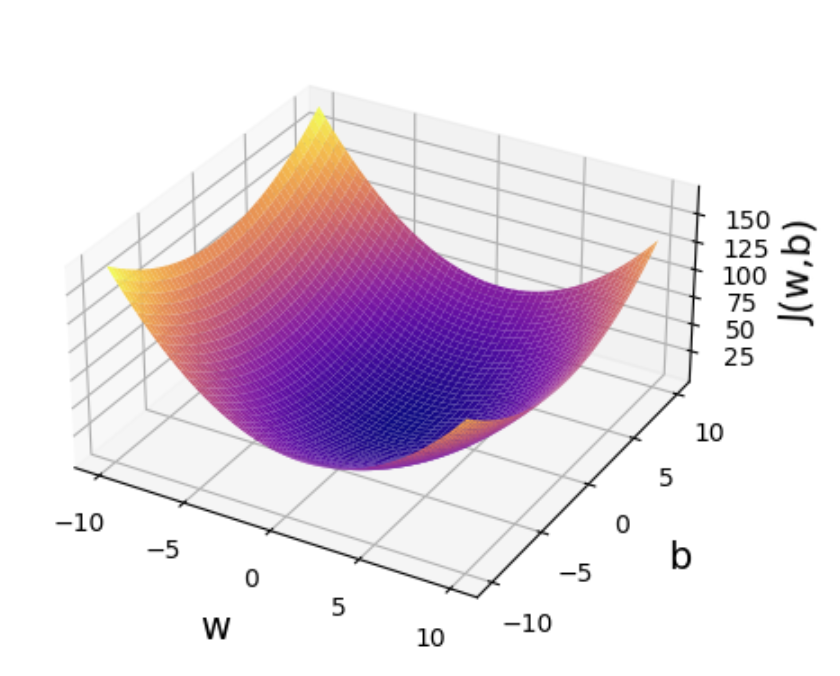
\includegraphics[width=\linewidth]{images/convex_loss.png}

{\scriptsize A convex loss surface $J(w,b)$ (e.g., squared error for linear regression).}
\end{column}

\begin{column}{0.6\textwidth}
\colorbox{yellow!30}{\textbf{Claim.}} If a function $f$ is convex, every local minimum of $f$ is a global minimum. \\
\vspace{0.5cm} 
\pause 
\colorbox{yellow!30}{\textbf{Proof sketch.}} By contradiction. Suppose $x^\star$ is a local minimum but not a global one. Then some $y$ has $f(y) < f(x^*)$. Convexity says $f$ lies below the chord on the segment from $x$ to $y$, so points on that segment arbitrarily close to $x^\star$ have values below $f(x)$. That contradicts $x$ being a local minimum. $\blacksquare$ \\
\vspace{0.5cm} 
\pause 
\colorbox{yellow!30}{\textbf{Who cares.}}  Linear regression and logistic regression have convex losses. This short contradiction argument guarantees that gradient descent can't get stuck at a bad solution on those models.\\
\end{column}
\end{columns}
\end{frame}





\begin{frame}[standout]
Group exercises
\end{frame}



\end{document}
